\chapter{Présentation, enjeux et attaques}
\label{chap:constantTimePresentation}


Ce premier chapitre a pour but de présenter les enjeux de la sécurité informatique face aux attaques par canal auxiliaire et d'introduire les attaques temporelles. Nous distinguerons ces attaques en deux catégories, montrant ainsi la diversité et les potentiels dangers pour un système sécurisé ignorant de cette menace.



\section{L'exécution du code est observable...}

L'Informatique repose sur deux fondations que nous tendons à distinguer dans l'enseignement : le matériel et le logiciel. Pourtant, si nous gardions séparé ces deux domaines, nous aurions des tas de piles de métal et de plastique d'un côté et des bibliothèques pleines d'idées intéressantes de l'autre. Au contraire, combiner les deux parties permet de réaliser des prouesses technologiques et scientifiques. Ainsi, lorsque nous concevons un système sécurisé, il nous faut prendre en compte ces deux composantes. Pour implémenter un système sécurisé, il ne faut pas seulement avoir un logiciel sécurisé, il est tout aussi important d'avoir un support physique sécurisé. Oublier ce détail, c'est oublier que programmer peut se résumer à manipuler de l'électricité.\medbreak

Les attaques par canal auxiliaires consistent à exploiter les caractéristiques matérielles du support pour gagner en connaissances sur un programme ciblé. Puis exploiter ces connaissances pour acquérir davantage d'informations privées : identifiants, clés secrètes, messages personnels. Nous leur attribuons le terme "canal auxiliaire" car il ne s'agit pas de trouver une faille perdue dans les limites d'un logiciel ou d'exploiter une mécanique du logiciel pour sortir de l'espace prévu par le concepteur. Il s'agit de se positionner hors du cadre de développement. Voici quelques travaux présentant une attaque par canal auxiliaire et le canal exploité :
\begin{itemize}
    \item[\cite{DPA_Attack}] Consommation d'énergie 
    \item[\cite{Branch_Attack}] Prédiction de branchement 
    \item[\cite{Thermal_Attack}] Variation de température
    \item[\cite{DRAM_Attack}] Accès à la mémoire DRAM
\end{itemize}\medbreak

Le point commun entre ces attaques est la nécessité d'avoir un point de contact avec la cible. Il faut que l'attaquant puisse récupérer le matériel informatique ou le programme qu'il souhaite attaquer pour ensuite poser des sondes/capteurs afin d'accumuler de la connaissance et mener son exploitation.\bigbreak


Une autre technique d'attaque consiste à venir introduire une erreur dans le déroulement normal d'un programme. Il s'agit d'une attaque par injection de faute. Originellement \cite{faultOverview} les fautes étaient "naturelles" : un défaut dans le code, un problème avec la transcription vers du code machine, un défaut d'un composant dans le système ou une interférence. Ces interférences sont causées par une irrégularité de l'alimentation électrique, des radiations électromagnétiques, une perturbation environnementale \etc\dots
En 2004, \citeauthor{Fault_Attacks} dans leur article \citetitle{Fault_Attacks} \cite{Fault_Attacks} effectuent un tour d'horizon des techniques, montrant l'efficacité de cette méthode sur \indexed{RSA}
% \footnote{Chiffrement asymétrique par clés secrètes du nom de ces auteurs. Standardisé en 1983.}
, \indexed{NVM}\footnote{Non Volatile Memory ou mémoire non volatile est un composant informatique qui conserve son contenu en l'absence d'électricité.}
, \indexed{DES}%\footnote{Algorithme de chiffrement symétrique par bloc. Standardisé en 1977}
, \indexed{EEPROM}\footnote{Electrically-Erasable Programmable Read-Only Memory ou mémoire morte effaçable électriquement et programmable.}, \indexed{JVM}\footnote{Machine virtuelle qui exécute des programmes compilés en bytecode Java.}. Nous retrouvons enfin une liste de contre-mesures et de méthodes de protection contre ces attaques.\medbreak

Ainsi, donner un accès physique à un inconnu est une porte d'entrée pour un attaquant. Pourtant, penser que l'accès physique au support est une condition nécessaire et suffisante pour réaliser une attaque par canal auxiliaire est une erreur.

\section{...à distance}

En effet, il est possible de réaliser des attaques à distance en exploitant d'autres failles de sécurité d'un programme ou d'autres caractéristiques matérielles. L'attaque présentée par \citeauthor{LLC_attack} dans \citetitle{LLC_attack} \cite{LLC_attack} repose sur la conception des services clouds où les machines virtuelles accèdent au même matériel. Tandis que la virtualisation crée l'illusion de compartimentation entre les sessions, en réalité, les adresses mémoire pointent vers une ressource physique partagée. Ainsi, l'exploitation du cache du dernier niveau (LLC) permet à un co-hôte de récupérer les clés secrètes d'un autre utilisateur. L'attaquant remplit le cache, puis mesure les temps d'accès vers ces registres, si des modifications apparaissent dans ces temps, cela signifie que la victime a accédé à ces registres. En répétant cette opération, l'attaquant peut reconstruire les clés secrètes de la victime.\medbreak


D'autres attaques distantes comme celle de \citeauthor{LLC_attack} existent \cite{cryptoeprint:2016/224,Moghimi_2017,vanbulck2018nemesis}, mais nous observons rapidement que ces techniques emploient aussi la méthode de chronométrage. En effet, si nous ciblons un algorithme et que nous mesurons son temps d'exécution, si en fournissant différentes entrées (considérées secrètes) des variations sont observées entre les mesures, alors cela signifie que l'algorithme présente une dépendance à ces entrées. Une sous-fonction de cet algorithme est généralement responsable de ces variations. Cette classe d'attaque est appelée <<\textit{attaque temporelle}>>\footnote{Le terme générique dans la recherche scientifique est <<\textit{time attack}>>. Une traduction plus précise serait <<\textit{attaque par chronométrage}>>. Nous choisissons ici d'utiliser le terme <<\textit{attaque temporelle}>> car il est moins lourd et renvoie directement vers la faille exploitée plutôt que par la méthode employée.}.\medbreak

Le lien entre temps et exécution de code est connu depuis le début de l'informatique. Le temps est le marqueur de performance, d'efficacité d'un programme. En revanche, l'idée d'exploiter cet indice pour réaliser une attaque est arrivée plus tardivement. \citeauthor{crypto-1996-1469} nous présente, le premier en 1996, comment monter une attaque en utilisant ce canal.\medbreak

Ce lien entre le temps et l'exécution du code est connu, pourtant la mesure de l'ampleur de la fuite d'information transmise par ce canal n'est pas triviale, ni à son époque, ni aujourd'hui.

\begin{listing}[!ht]
    \caption{Exemple de code vulnérable à une attaque temporelle}
    \label{lst:timing_attack_example}
    \begin{minted}[frame=lines,framesep=2mm,baselinestretch=1.2,fontsize=\footnotesize,linenos, gobble=6]{C}
        bool check_pwd(msg, pwd){
        if (msg.length != pwd.length){
            return False
        }
        for(int i = 0; i < msg.length; i++){
            if(msg[i] != pwd[i]){
                return False
            }
        }
        return True
        }
    \end{minted}
\end{listing}
                
Si nous prenons les instructions présentent dans le code \ref{lst:timing_attack_example}, nous pouvons observer que la fonction \texttt{check\_pwd} compare deux chaînes de caractères. Si elles sont de même longueur, elle les compare caractère par caractère. Si elles sont de longueur différentes, la fonction retourne immédiatement \texttt{False}. Ainsi, si nous fournissons un mot de passe de longueur différente, le temps d'exécution sera constant et court. En revanche, si nous fournissons un mot de passe de même longueur, le temps d'exécution dépendra du nombre de caractères identiques consécutifs entre les deux chaînes. En effet, la fonction s'arrêtera dès qu'un caractère différent est trouvé. Ainsi, en mesurant le temps d'exécution pour différents mots de passe, un attaquant peut déduire des informations sur le mot de passe correct.\medbreak

Nous pouvons synthétiser les exécutions de la fonction \texttt{check\_pwd} en un graphe comme celui présenté par la figure \ref{fig:timing_attack_example}. Chaque interruption de la fonction peut être observée et mesurée, permettant ainsi de régénérer le mot de passe. Bien sûr, la connaissance du protocole ciblé est requise, ou alors il faut réaliser un travail de rétro-ingénierie pour calibrer l'attaque.\medbreak

\begin{figure}[!ht]
    \caption{Suivi du temps d'exécution pour différents mots de passe}
    \label{fig:timing_attack_example}
    \center
    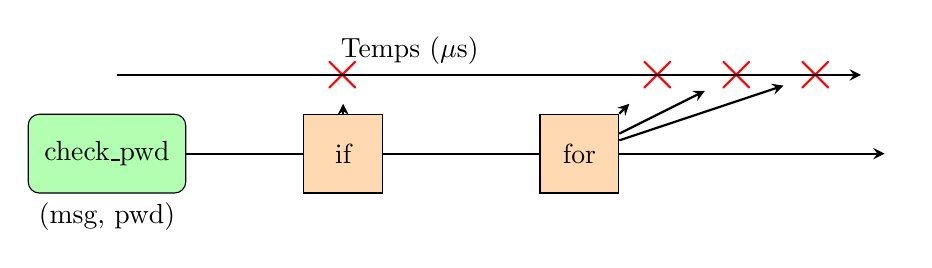
\begin{tikzpicture}[auto]

    % Styles
    \tikzstyle{startstop} = [rectangle, rounded corners, minimum width=2cm, minimum height=1cm, text centered, draw=black, fill=green!30]
    \tikzstyle{process} = [rectangle, minimum width=1cm, minimum height=1cm, text centered, draw=black, fill=orange!30]
    \tikzstyle{arrow} = [thick,->,>=stealth]
    \tikzstyle{arrowred} = [thick,->,>=stealth, draw=red]
    
    % Noeuds
    \node (start) [startstop] {check\_pwd};
    \node (valid) [right of=start, xshift=9cm, green] {\huge{$\checkmark$}};
    \draw [arrow] (start) -- (valid);
    
    \node (inputs) [below of = start, yshift=0.2cm] {(msg, pwd)};
    \node (if) [process] [right of=start, xshift=2cm] {if};
    \node (not) [above of=if, red] {\huge{$\times$}};
    \node (for) [process] [right of=if,, xshift=2cm] {for};
    \node (for1) [above of=for,xshift=1cm, red] {\huge{$\times$}};
    \node (for2) [right of=for1, red] {\huge{$\times$}};
    \node (for3) [right of=for2, red] {\huge{$\times$}};

    \draw [arrow] (if) -- (not);
    \draw [arrow] (for) -- (for1);
    \draw [arrow] (for) -- (for2);
    \draw [arrow] (for) -- (for3);

    \node (t) [above of=start] {};
    \node (a) [above of=valid, xshift=-0.3cm] {};
    \draw [arrow] (t) -- node[above left] {Temps ($\mu$s)} (a.west);
    
    \end{tikzpicture}
\end{figure}

Cette méthode est plus efficace qu'une attaque par force brute. En effet, si le mot de passe est composé de 8 caractères de l'alphabet latin, alors il y a 256 possibilités par caractère, pour un total de $256^8 = 2^{64}$ possibilités. En revanche, si nous utilisons la méthode de l'attaque temporelle, le nombre de possibilités est réduit à $8 + 8 \times 256 = 2056$ possibilités. En effet, nous cherchons dans un premier temps à identifier la longueur du mot de passe, puis nous identifions ensuite caractère après caractère pour trouver le mot de passe. Des temps d'exécution courts correspondent à des cas d'échec, tandis qu'un allongement du temps d'exécution nous permet de déterminer une bonne piste.\medbreak

Les attaques temporelles présentent la particularité d'être génériques. Tandis que les attaques décrites précédemment nécessitent des conditions d'accès ou d'initialisation plus importantes, cette classe d'attaque présente l'avantage d'être réalisable sur tous les types de systèmes, et notamment les systèmes accessibles par internet. La connaissance de cette menace est donc primordiale pour l'implémentation et la mise en service de produits sur Internet.\medbreak

Par la suite du document, le terme "fuite" sera utilisé pour désigner un extrait du programme qui peut être exploité pour réaliser une attaque temporelle. Si nous reprenons le code \ref{lst:timing_attack_example}, les branchements conditionnels lignes [4, 6] sont des fuites d'informations. C'est grâce à ces instructions que l'attaque décrite précédemment est réalisable.\medbreak

\vfill
\textit{Nous allons maintenant nous intéresser aux moyens et méthodes à notre disposition pour nous protéger contre les attaques temporelles.}



